%% LyX 2.4.0~RC3 created this file.  For more info, see https://www.lyx.org/.
%% Do not edit unless you really know what you are doing.
\documentclass[twocolumn,spanish,aps,prl,groupedaddress]{revtex4-2}
\usepackage[T1]{fontenc}
\usepackage[utf8]{inputenc}
\setcounter{secnumdepth}{3}
\usepackage{amsmath}

\makeatletter
%%%%%%%%%%%%%%%%%%%%%%%%%%%%%% User specified LaTeX commands.
\usepackage{graphicx}
\usepackage{epstopdf}
%\usepackage{amsmath}% http://ctan.org/pkg/amsmath
%\usepackage{amsthm}
%\usepackage{amsfonts}
%\usepackage{subfigure}
%\usepackage{hhline}
%\usepackage[miktex]{gnuplottex}
%\usepackage{xcolor}
\usepackage{amssymb}
\usepackage{amsmath}
\usepackage{color}
\usepackage{hyperref}
%\usepackage[percent]{overpic}
\usepackage{tikz}
\usepackage{mathrsfs}
\usepackage{wasysym}
\usepackage{tikz-cd}
%\usepackage{stix} %\fisheye
\usepackage{stackengine,scalerel}

% so sections, subsections, etc. become numerated.
\setcounter{secnumdepth}{3}

\newcommand{\avrg}[1]{\left\langle #1 \right\rangle}
\newcommand{\nelta}{\bar{\delta}}
\newcommand{\bra}[1]{\left\langle #1\right|}
\newcommand{\ket}[1]{\left| #1 \right\rangle}
\newcommand{\sbra}[1]{\langle #1|}
\newcommand{\sket}[1]{| #1 \rangle}
\newcommand{\bek}[3]{\left\langle #1 \right| #2 \left| #3 \right\rangle}
\newcommand{\sbek}[3]{\langle #1 | #2 | #3 \rangle}
\newcommand{\braket}[2]{\left\langle #1 \middle| #2 \right\rangle}
\newcommand{\ketbra}[2]{\left| #1 \middle\rangle \middle\langle #2  \right|}
\newcommand{\sbraket}[2]{\langle #1 | #2 \rangle}
\newcommand{\sketbra}[2]{| #1 \rangle  \langle #2 |}
\newcommand{\norm}[1]{\left\lVert#1\right\rVert}
\newcommand{\snorm}[1]{\lVert#1\rVert}
\newcommand{\bvec}[1]{\boldsymbol{\mathsf{#1}}}
\newcommand{\bcov}[1]{\boldsymbol{#1}}
\newcommand{\bdua}[1]{\boldsymbol{\check{#1}}}
%\newcommand{\bdov}[1]{\boldsymbol{\breve{#1}}}
\newcommand{\bdov}[1]{\breve{#1}}
%\newcommand{\bten}[1]{\boldsymbol{\mathfrak{#1}}}
\newcommand{\bten}[1]{\boldsymbol{\mathfrak{#1}}}
\newcommand{\forany}{\tilde{\forall}}
\newcommand{\qed}{$\overset{\circ}{.}\;$}

\newcommand\bigeye{\ensurestackMath{\stackinset{c}{}{c}{-.3pt}%
  {\bullet}{\scriptstyle\bigcirc}}}
\newcommand\eye{\scalerel*{\bigeye}{x}}
%\newcommand*{\fisheye}{%
%    \mathbin{%
%        \ooalign{$\circledcirc$\cr\hidewidth$\bullet$\hidewidth}%
%    }%
%}
\renewcommand{\appendixname}{Apéndice} % Change "Appendix" to "Apéndice"
\renewcommand{\fnum@figure}{Fig.~\thefigure} 

\makeatother

\usepackage{babel}
\addto\shorthandsspanish{\spanishdeactivate{~<>.}}
\deactivatequoting

\begin{document}
\title{Modelo Hodgkin \& Huxley}
\author{Adolfo Banchio}
\email{adolfo.banchio@mi.unc.edu.ar}

\author{Alejandro Matias Toledo}
\email{amtoledo@mi.unc.edu.ar}

\affiliation{Facultad de Matemática, Astronomía, Física y Computación, Universidad
Nacional de Córdoba}
\date{\today}
\begin{abstract}
En este trabajo se estudia el comportamiento de una neurona desde
un enfoque teórico, utilizando el modelo matemático de Hodgkin y Huxley.
Este modelo describe la propagación del potencial de acción a partir
del funcionamiento de los canales iónicos en la membrana neuronal.
Se realizaron simulaciones numéricas del modelo para analizar propiedades
clave del potencial de acción. Este trabajo es importante para comprender
los mecanismos fundamentales de la excitación neuronal y su propagación.
\end{abstract}
\maketitle

\section{INTRODUCCION}

Las neuronas son las células encargadas de transmitir la información
en organismos complejos a través de señales electricas, estos mensajes
se conocen como el potencial de acción. Nace en la propia neurona
y se va propagando de una a otra hasta alcanzar el destino objetivo,
este sera nuestro objeto de estudio para este trabajo. Lo estudiaremos
a partir del modelo propuesto por Hodgking y Huxley en el año 1952
realizando simulaciones numericas del sistema, con el objetivo de
estudiar la celula desde un punto de vista de un sistema dinamico.
Buscaremos contestar preguntas como <<¿Que hace disparar una neurona?>>
o <<¿Cual es el umbral?>>~\cite{HodgkinHuxleyModel}~\cite{izhikevich2006}

\section{TEORÍA}

El modelo de H\&H propuesto trata de explicar el funcionamiento de
la neurona como capacitores donde la diferencia de potencial eléctrico
entre el exterior y el interior se da debido a diferentes concentraciones
de cargas iónicas. Considerando que las neuronas poseen dos canales,
uno de sodio con dos compuertas (entrada y salida) y otro de potasio
con una única compuerta. El sistema puede ser descripto por las siguientes
ecuaciones diferenciales. {\small\begin{eqnarray*}
\dot{n}&=&\alpha_n(v)(1-n)-\beta_n(v) n\\
\dot{m}&=&\alpha_m(v)(1-m)-\beta_m(v) m\\
\dot{h}&=&\alpha_h(v)(1-h)-\beta_h(v) h \\
\dot{v}&=&c^{-1}(i-\bar{g}_{\mathrm{Na}}m^3h(v-v_{\mathrm{Na}})-\bar{g}_{\mathrm{K}}n^4(v-v_{\mathrm{K}})-g_{l}(v-v_{l}))
\end{eqnarray*}}{\small\par}

Donde n representa la fraccion de compuertas de potasio abiertas,
m la fraccion de compuertas de activación de sodio abiertas y h la
fraccion de compuertas de inactivación abiertas. Para cada caso $\alpha_{k}$
y $\beta_{k}$ representan la tasa de apertura y clausura de cada
tipo de compuerta respectivamente;v representa el potencial electrico
de la membrana neuronal e i la corriente externa que estimula a la
neurona. Las ecuaciones y valores de los parametros estan desarrollados
en ~\cite{izhikevich2006}.

En este trabajo integraremos numericamente dichas ecuaciones en pos
de poder representar el comportamiento del sistema bajo el estimulo
de diferentes corrientes externas. 

\section{RESULTADOS}

El primero de los analisis realizados fue encontrar los valores de
equilibrio de las cuatro variables involucradas en nuestro sistema.
Para ello integramos numericamente partiendo desde una condicion inicial
de 0 para cada variable. ver fig.~\ref{fig:fig1} a. En general los
siguientes escenarios simulados partiran desde la condicion inicial
de los valores de equilibrio y variaran la funcion que representa
la corriente externa del sistema.

\subsection{Estimulo debil y estimulo fuerte}

La corriente externa introducida en este escenario estaba representada
por la siguiente funcion:

$i(t)=\begin{cases}
10\mu A/cm^{2} & t\in[2ms,2.5ms]\\
30\mu A/cm^{2} & t\in[10ms,10.5ms]\\
0 & c.c
\end{cases}$

Los resultados obtenidos se pueden ver en el siguiente grafico.~\ref{fig:fig1} b
Podemos notar que en el primer impulso, en t=2ms, se produce un estimulo
debil que no es suficiente para que la neurona se active. En cambio,
en el segundo impulso, en t=10ms, se produce un estimulo mas potente
que se observa que es suficiente para que la neurona se active y dispare. 

Ahora bien, con respecto a las compuertas, observamos que en el impulso
de t=2ms la fraccion de canales de sodio activados m y la fracción
de canales de sodio inactivados h se activan y desactivan rápidamente,
respectivamente, en cambio, la fracción de canales de potasio activados
n se activa lentamente. Todas las compuertas vuelven en poco tiempo
a su estado inicial. 

Luego, en el impulso de t=10ms, la fracción de canales de sodio activados
m y la fracción de canales de sodio inactivados h se activan y desactivan
rápidamente, respectivamente. Y la fracción de canales de potasio
activados n se activa en menor escala, pero se mantiene activada por
un tiempo mas prolongado ya que el estimulo es mas potente, que provoca
que la neurona se active y dispare, una vez que el estimulo pasa,
las compuertas vuelven a su estado inicial, en un tiempo menor pero
cercano al periodo refractario.

\subsection{Ráfaga}

La corriente externa se daba por:

$i(t)=\begin{cases}
10\mu A/cm^{2} & t\in[5ms,\infty ms]\\
0 & c.c.
\end{cases}$

Resultados ~\ref{fig:fig2}. Podemos observar que la neurona se activa
y dispara en el tiempo de estimulo (a partir de t=5ms), y luego se
mantiene en un estado de rafaga, ya que el estimulo es constante. 

En cuanto a las compuertas, una vez iniciado el sistema, tienden a
su estado de equilibrio, tambien observamos que la fracción de canales
de sodio activados y la fracción de canales de sodio inactivados se
abren y cierran rápidamente, respectivamente, en cambio, la fracción
de canales de potasio activados n se abren lentamente.

Una vez disparado (ya que el estimulo es suficiente para que la neurona
dispare), las compuertas tienden a volver a su estado inicial, pero
como es un estimulo constante, una vez pasado el periodo refractario,
la neurona vuelve a disparar, repitiendo nuevamente el proceso antes
descripto.

\subsection{Período Refractario}

La corriente externa se da por:
\begin{flushleft}
$i(t)=\begin{cases}
10\mu A/cm^{2} & t\in[10ms,10ms\:k+2],k\in\{1,2,3,4,..\}\\
0 & c.c.
\end{cases}$
\par\end{flushleft}

Ver resultados~\ref{fig:fig3}. En este caso podemos observar que
la corriente no es continua como el caso anterior, sino que el estimulo
se produce en intervalos de tiempo de 2ms, y luego se mantiene en
8ms sin estimulo. En el primer estimulo, sucede un potencial de acción,
causando los efectos sobre las compuertas ya conocidas. Luego observamos
que en el periodo refractario luego de la activación, la neurona es
incapaz de generar otro potencial de acción, incluso si recibe un
estímulo. 

Observamos que durante el período refractario, la compuerta h permanece
cerrada durante la despolarización. Esto significa que los canales
de sodio no se pueden abrir, impidiendo el aumento del potencial.
La compuerta n, por otro lado, puede estar abierta o cerrada, dependiendo
de la fase del período refractario:
\begin{itemize}
\item Período refractario absoluto: Todas las compuertas h están cerradas,
imposibilitando completamente la generación de un nuevo potencial
de acción.
\item Período refractario relativo: Algunas compuertas h comienzan a abrirse,
por lo que es posible generar un potencial de acción si el estímulo
es lo suficientemente fuerte para superar la hiperpolarización causada
por el flujo de iones de potasio a través de las compuertas n abiertas.
\end{itemize}
Analizando los graficos de sodio y potasio,durante el periodo refractario,
la cantidad de sodio dentro de la neurona disminuye luego del pico
del potencial de acción. Esto se debe a que, tras la despolarización,
la compuerta h se cierra, impidiendo la entrada de más iones de sodio.
Aunque un estímulo débil pueda causar una pequeña despolarización
local, no será suficiente para abrir las compuertas m de los canales
de sodio, por lo que no habrá un flujo masivo de sodio hacia el interior
de la neurona

La cantidad de potasio dentro de la neurona durante el periodo refractario
es menor que en reposo. La apertura de las compuertas n durante la
fase descendente del potencial de acción permite la salida de iones
de potasio, contribuyendo a la repolarización e incluso a la hiperpolarización.
Un estímulo débil durante el periodo refractario no alterará significativamente
este flujo de potasio, ya que la mayoría de las compuertas n ya estarán
abiertas o en proceso de abrirse.

En este caso, podemos observar que el estimulo no es lo suficientemente
fuerte para que la neurona genere un potencial de acción en el período
refractario. 

En resumen, el período refractario es una consecuencia directa del
comportamiento de las compuertas iónicas, especialmente el cierre
de la compuerta h, que impide la apertura de los canales de sodio
y la generación de un nuevo potencial de acción. Este mecanismo asegura
que los potenciales de acción se propaguen en una sola dirección y
limita la frecuencia máxima de disparo de la neurona.

\subsection{Exitaciones con ruido}

En este caso la corriente es estocastica tal que $i(t)\sim i_{0}N(0,1)$
donde establecemos $i_{0}=50$. Y los resultados obtenidos para este
caso se ven en fig ~\ref{fig:fig4}. 

bla bla bla analissis analisis

\section{DISCUSIÓN}

\section{CONCLUSIONES}

\section{AGRADECIMIENTOS}

\bibliographystyle{apsrev4-2}
\bibliography{ref}

\begin{figure}[htbp]
  \centering
  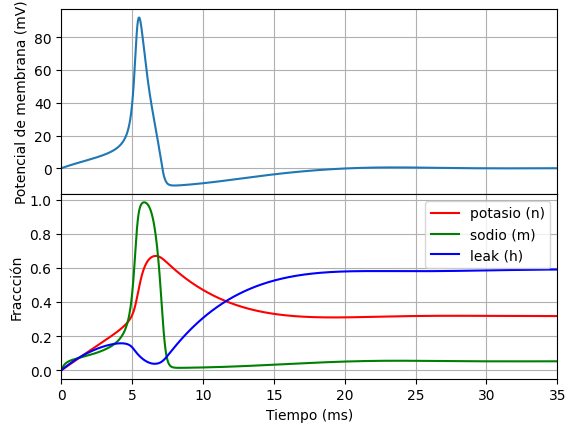
\includegraphics[width=0.5\textwidth]{graficos/ejercicio_3.png}
  \put(-240,140){\bf a)}
  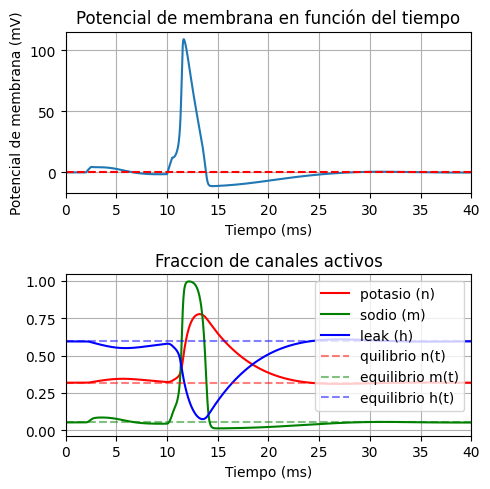
\includegraphics[width=0.5\textwidth]{graficos/ejercicio_4.png}
  \put(-240,140){\bf b)}
  \caption{
    \label{fig:fig1}
    Comparación entre dos imágenes. \\
    {\bf a)} Descripción de la primera imagen.
    {\bf b)} Descripción de la segunda imagen.
  }
\end{figure}

\begin{figure}[htbp]
  \centering
  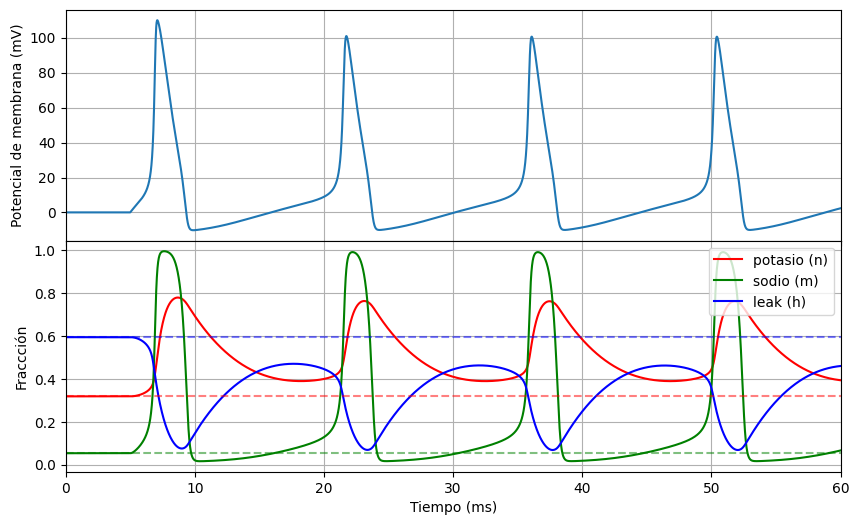
\includegraphics[width=0.90\textwidth]{graficos/ejercicio_5.png}
  \caption{Gráfico 1: Nombre o descripción del gráfico 5.}
  \label{fig:fig2}

  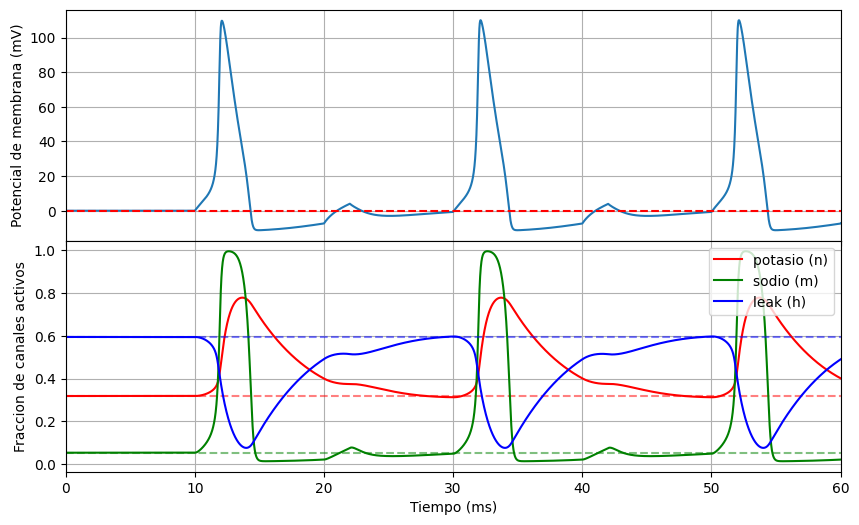
\includegraphics[width=0.90\textwidth]{graficos/ejercicio_6.png}
  \caption{Gráfico 1: Nombre o descripción del gráfico 6.}
  \label{fig:fig3}
\end{figure}

\begin{figure}[htbp]
  \centering
  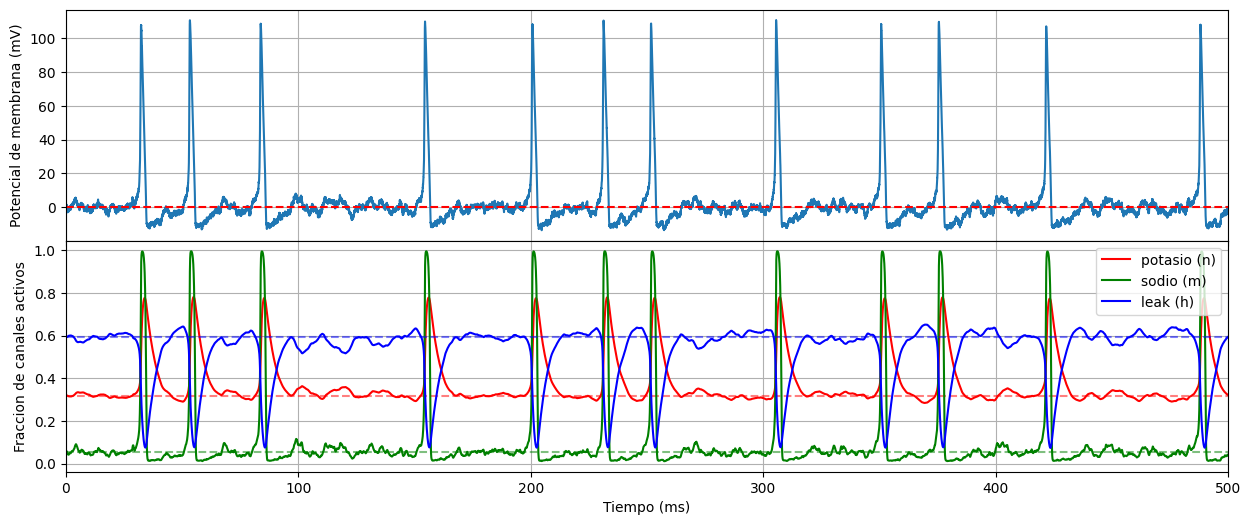
\includegraphics[width=0.9\textwidth]{graficos/ejercicio_7.png}
  \caption{Gráfico 1: Nombre o descripción del gráfico 7.}
  \label{fig:fig4}
\end{figure}
\end{document}
